\documentclass[../main.tex]{subfiles}
\begin{document}

\chapter{Metodología}\label{ch:metodologia}

\section{Metodología de trabajo}

En la gestión de este proyecto se ha utilizado la metodología \textbf{Kanban}.

Kanban se basa en la idea de que el trabajo que se está realizando debe limitarse y solamente se debe empezar algo cuando un bloque de trabajo anterior haya sido entregado o ha pasado a otra función posterior de la cadena.\cite{Ahmad2013}

Esta metodología utiliza un mecanismo de control visual para hacer seguimiento del trabajo conforme este va recorriendo el flujo de valor. Este mecanismo se ha basado en un tablero en el software de gestión de proyectos \textbf{Trello}\cite{JohnsonMLIS2017}.

La correspondencia entre la metodología de trabajo y el tablero de Trello será:

Las \textbf{tareas} en las que se desgrana el proyecto serán \textit{tarjetas}. Estas tarjetas tendrán un nombre significativo, u  miembro responsable, una descripción, una etiqueta que indique el nivel de prioridad (baja o urgente) y la naturaleza (Pruebas, Búsqueda, Desarrollo o Escritura) de la tarea, una fecha de vencimiento que indicará la fecha máxima para completar la tarea y un conjunto de comentarios para que los miembros del equipo puedan comentar aspectos referentes a esa tarea.

Los \textbf{estados} por los que puede pasar una tarea serán listas. Estas listas son:
\begin{itemize}
    \item\textbf{ Pendiente}: Estado inicial de todas las tareas de carácter general. Es necesario indicar el miembro al que le corresponde una tarea, así como una fecha límite para completarla.
    \item \textbf{En desarrollo}: Cuando se ha iniciado el proceso de una tarea, esta pasa a \textit{En Desarrollo}.
    \item \textbf{Revisión}: Estado que indica que la tarea se ha completado pero necesita una revisión por parte de otro miembro del equipo. Se asignará la tarea a quién corresponda su revisión.
    \item \textbf{Finalizado}: Estado final de la tarea que indica que ya se han terminado todos los trabajos referentes a ella. Solamente podrá pasar la tarea a finalizado el responsable de su revisión.
    \item \textbf{[Dev] Pendiente}: Estado inicial de las tareas que implican un desarrollo de código. Funciona de la misma forma que la anterior columna de \textit{Pendiente}.
    \item \textbf{[Dev] En Desarrollo}: Cuando se ha iniciado el proceso de una tarea que estaba en \textit{[Dev] Pendiente} se pasará a esta columna.
    \item \textbf{[Dev] Hecho}: Una vez finalizada la tarea, se pasará a este estado marcándola como finalizada.
\end{itemize}

En este tablero existe una columna adicional llamada \textit{Documentos} donde se almacenan documentos y enlaces importantes del proyecto.

\begin{figure}[H]
    \centering
    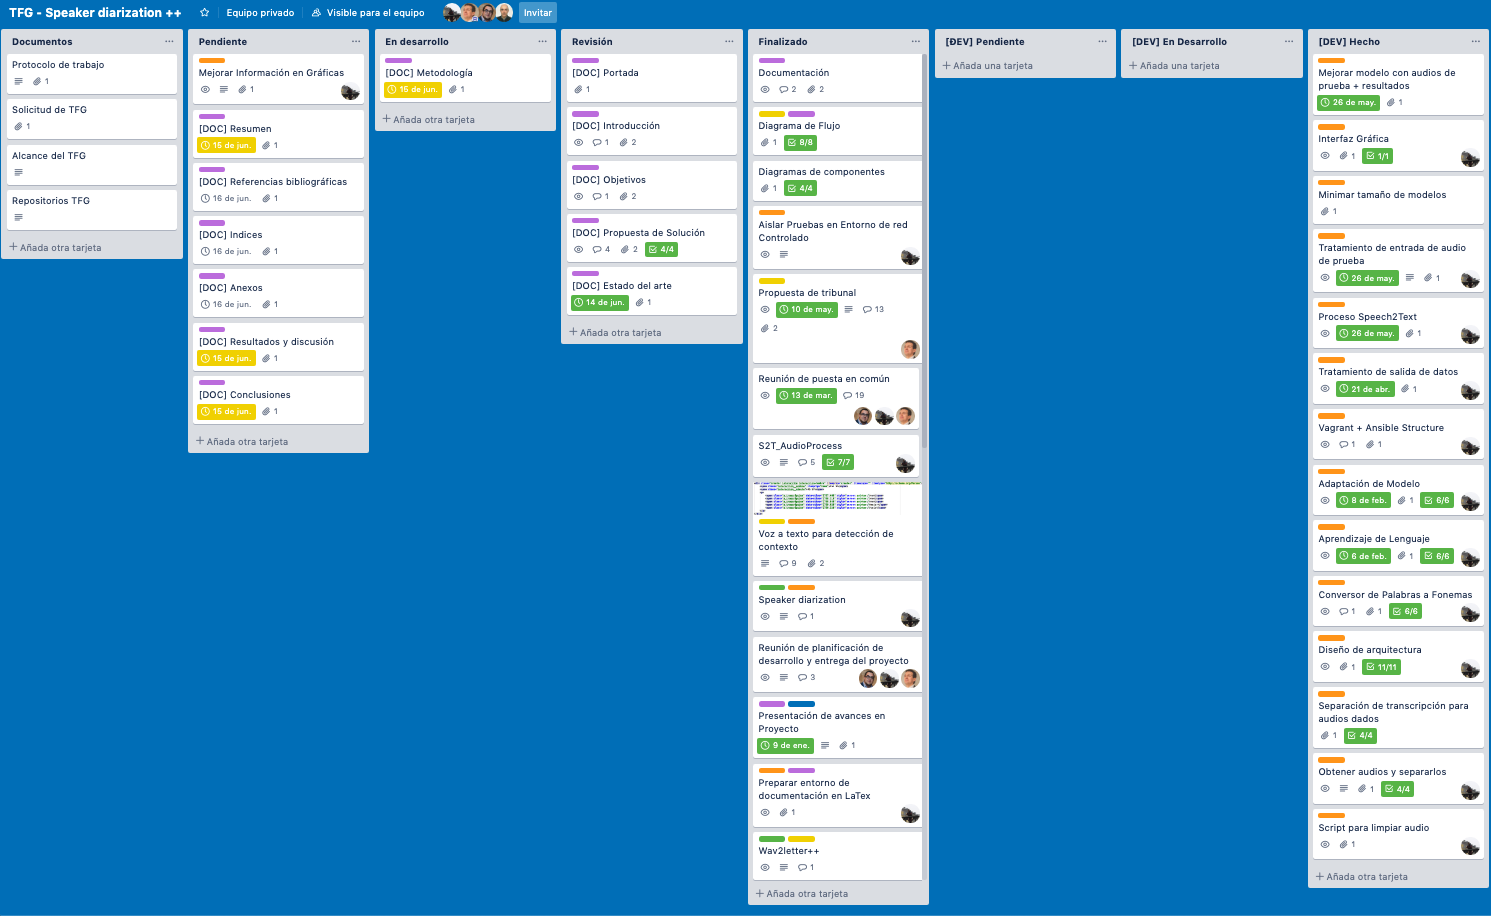
\includegraphics[width=0.7\textwidth]{trello}
    \caption{Tablero de Trello del proyecto.}
    \label{img:trello}
\end{figure}

\section{Planificación}
El proyecto tuvo una \textbf{planificación inicial} de 300 horas de trabajo que se dividieron en: Investigación (30 horas), Diseño y Análisis de la Solución (65 horas), Implementación de la Solución (150 horas), Validación de la Solución (15 horas) y Documentación (40 horas).

Conforme el proyecto fue avanzando, la estimación inicial se incumplió teniendo así un reparto de horas de la siguiente forma: Investigación (77,50 horas), Diseño y Análisis de la Solución (26,74 horas), Implementación de la Solución (303,58 horas), Validación de la Solución (34,12 horas) y Documentación (142,78 horas).

\begin{table}[H]
    \centering
    \resizebox{\textwidth}{!}{%
    \begin{tabular}{|l|c|c|c|c|c|c|}
        \hline
        \textbf{Tareas principales} & \multicolumn{1}{l|}{\textbf{Tiempo estimado {[}h{]}}} & \multicolumn{1}{l|}{\textbf{Total tiempo estimado {[}h{]}}} & \multicolumn{1}{l|}{\textbf{Tiempo dedicado {[}h{]}}} & \multicolumn{1}{l|}{\textbf{Total tiempo dedicado {[}h{]}}} & \multicolumn{1}{l|}{\textbf{Diferencia {[}h{]}}} & \multicolumn{1}{l|}{\textbf{Diferencia Total {[}h{]}}} \\ \hline
        \textbf{Investigación} & 30 &  & 77,50 &  & \cellcolor[HTML]{FFCCC9}+47,5 & \cellcolor[HTML]{FFCCC9} \\ \cline{1-2} \cline{4-4} \cline{6-6}
        \textbf{Diseño y Análisis de Solución} & 65 &  & 26,74 &  & \cellcolor[HTML]{9AFF99}{\color[HTML]{333333} -38,26} & \cellcolor[HTML]{FFCCC9} \\ \cline{1-2} \cline{4-4} \cline{6-6}
        \textbf{Implementación/Desarrollo} & 150 &  & 303,58 &  & \cellcolor[HTML]{FFCCC9}+153,58 & \cellcolor[HTML]{FFCCC9} \\ \cline{1-2} \cline{4-4} \cline{6-6}
        \textbf{Validación} & 15 &  & 34,12 &  & \cellcolor[HTML]{FFCCC9}+19,12 & \cellcolor[HTML]{FFCCC9} \\ \cline{1-2} \cline{4-4} \cline{6-6}
        \textbf{Documentación} & 40 & \multirow{-5}{*}{300} & 142,78 & \multirow{-5}{*}{584,72} & \cellcolor[HTML]{FFCCC9}{\color[HTML]{333333} +102,78} & \multirow{-5}{*}{\cellcolor[HTML]{FFCCC9}+284,72} \\ \hline
    \end{tabular}%
    }
    \caption{Comparativa de horas estimadas y horas dedicadas al desarrollo del proyecto.}
    \label{tab:horas}
\end{table}

Como observamos en la \autoref{tab:horas} existe un gran descompensación entre las horas planificadas y las horas dedicadas (más de 284 horas). Esta descompensación se basa en el crecimiento del proyecto a medida que se ha ido desarrollando ya que se deseaban cumplir todos los objetivos marcados.

Este registro de tiempo se ha realizado utilizando la herramienta \textbf{Harvest}\cite{harvest}. Este software en línea permite registrar el tiempo de trabajo por cada tarea definida anteriormente en Trello. Por tanto, una vez acabado el proyecto se ha podido estudiar el tiempo dedicado en cada una de las tareas definidas.

\section{Gestión de código fuente}
El código fuente del proyecto se ha gestionado a través de repositorios privados de códigos en la plataforma \textbf{GitHub}\cite{github}. GitHub es una plataforma para almacenar proyectos utilizando el sistema de control de versiones \textbf{Git}\cite{Somasundaram2013}. Utilizar un sistema de control de versiones facilita las tareas de mantenimiento del código ya que cada versión que se genere del proyecto se almacenará estando siempre disponible.

Para este proyecto se han creado nueve \textbf{repositorios}: Un repositorio general que contiene a los demás repositorios del proyecto y al código fuente encargado del despliegue de la infraestructura de ejecución, y a ocho repositorios que se corresponden con los componentes del sistema explicados en la \autoref{subsec:arquitectura_sistema}. Estos repositorios de componentes contendrán el código fuente e información de despliegue en contenedores.

El repositorio principal está conectado a los repositorios de los componentes con \textit{Submódulos}. Esto permite que aunque exista un repositorio principal, se puedan mantener un control de versiones de cada componente de forma independiente.

De manera adicional y para crear una conexión normalizada entre la gestión de tareas y las gestión de versiones se ha utilizado el modelo de ramificaciones \textbf{GitFlow}. Este modelo se basa en el uso de las ramas en Git para gestionar las versiones en desarrollo o completadas. Las distintas ramas existentes son:
\begin{itemize}
    \item Rama \textit{master}: Rama principal donde se encuentran versiones del proyecto totalmente funcionales.
    \item Rama \textit{develop}: Rama de trabajo donde se encuentra el código que formará una versión que posteriormente se trasladará a \textit{master}.
    \item Ramas tipo \textit{feature}: Ramas que parten de la rama \textit{develop} y se utilizan para desarrollar una determinada característica de la aplicación. Cuando se termine el trabajo, esta rama se fusionará con \textit{develop} de nuevo. 
\end{itemize}
Aunque existen ramas de tipos \textit{hotfix} y \textit{release} no se han utilizado debido a que el proyecto no lo requería.

En este proyecto se ha trabajado siguiendo un protocolo con las herramientas antes comentadas: Cuando una tarea esta \textit{[Dev] Pendiente} y se empieza a desarrollar, su respectiva tarjeta en Trello se mueve a la columna \textit{[Dev] En desarrollo}. En este momento se crea una rama \textit{feature} en el repositorio del proyecto correspondiente. Una vez la tarea se ha finalizado, la tarjeta de Trello pasa a la columna \textit{[Dev] Finalizado} y la rama creada se fusiona con la rama \textit{develop} resolviendo algunos conflictos que puedan haber sucedido.

Los repositorios con los enlaces a GitHub son:
\begin{itemize}
    \item \textbf{S2T}: \href{https://github.com/pamamu/S2T}{https://github.com/pamamu/S2T}
    \item \textbf{S2T\_AudioProcess}: \href{https://github.com/pamamu/S2T_AudioProcess}{https://github.com/pamamu/S2T\_AudioProcess}
    \item \textbf{S2T\_G2P}: \href{https://github.com/pamamu/S2T_G2P}{https://github.com/pamamu/S2T\_G2P}
    \item \textbf{S2T\_GetAudioTrans}: \href{https://github.com/pamamu/S2T_GetAudiosTrans}{https://github.com/pamamu/S2T\_GetAudiosTrans}
    \item \textbf{S2T\_MainController}: \href{https://github.com/pamamu/S2T_MainController}{https://github.com/pamamu/S2T\_MainController}
    \item \textbf{S2T\_SPHINXBASE}: \href{https://github.com/pamamu/S2T_SPHINXBASE}{https://github.com/pamamu/S2T\_SPHINXBASE}
    \item \textbf{S2T\_SRILM}: \href{https://github.com/pamamu/S2T_SRILM}{https://github.com/pamamu/S2T\_SRILM}
    \item \textbf{S2T\_Speech2Text}: \href{https://github.com/pamamu/S2T_Speech2Text}{https://github.com/pamamu/S2T\_Speech2Text}
    \item \textbf{S2T\_Training}: \href{https://github.com/pamamu/S2T_Training}{https://github.com/pamamu/S2T\_Training}
\end{itemize}

De manera adicional se ha creado un repositorio para almacenar la documentación realizada en \LaTeX: \href{https://github.com/pamamu/S2T_OfficialDocumentation}{https://github.com/pamamu/S2T\_OfficialDocumentation}.


\end{document}